\documentclass[aspectratio=169]{beamer}
\usepackage[utf8]{inputenc}
\usepackage{lmodern}
\usepackage{tikz}
\usepackage{hyperref}
\definecolor{pbprimary}{HTML}{F4A261}
\definecolor{pbsecondary}{HTML}{FFE8B6}
\setbeamercolor{palette primary}{bg=pbprimary, fg=white}
\setbeamercolor{frametitle}{fg=pbprimary}
\setbeamercolor{title}{fg=pbprimary}
\setbeamercolor{block title}{bg=pbprimary, fg=white}
\setbeamercolor{block body}{bg=pbsecondary, fg=black}
\setbeamercolor{alertblock title}{bg=pbprimary, fg=white}
\setbeamercolor{alertblock body}{bg=pbsecondary!80, fg=black}
\setbeamertemplate{navigation symbols}{}
\setbeamertemplate{itemize item}{\color{pbprimary}\Large$\blacktriangleright$}
\title{Technology in the Workplace}
\subtitle{Student Guide Deck}
\author{Pine Brook IGNITE}
\date{Spring 2026}
\begin{document}
\begin{frame}[plain]
\begin{center}
{\usebeamerfont{title}\color{pbprimary}\Huge Technology in the Workplace\par}
\vspace{0.3cm}
{\Large Today we will learn, build, test, and show our thinking.\par}
\vspace{0.35cm}
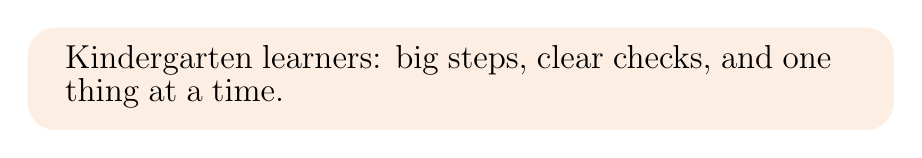
\begin{tikzpicture}
\fill[pbprimary!18, rounded corners=10pt] (0,0) rectangle (11,1.3);
\node[anchor=west, text width=10.2cm] at (0.35,0.68) {\large Kindergarten learners: big steps, clear checks, and one thing at a time.};
\end{tikzpicture}
\end{center}
\end{frame}
\begin{frame}{Todays Goal}
\begin{itemize}
\item I can identify jobs that use technology (K-1.IC.7)
\item I can talk about how technology is helpful to different jobs (K.1C.7)
\item I can find computing technology used in different places (classroom, home, and community). (K-1.IC.3)
\end{itemize}
\begin{block}{Remember}
We do not have to be perfect right away. We take one step, then the next step, then we check.
\end{block}
\end{frame}
\begin{frame}{What You Need}
\begin{itemize}
\item Your class materials
\item The digital tool or build materials for today
\item A partner voice and your thinking
\end{itemize}
\begin{block}{Partner Norms}
Look. Listen. Try. Talk. Help without taking over.
\end{block}
\end{frame}
\begin{frame}{Step 1}
\begin{block}{Listen for the key idea and connect it to real life.}
Listen for the key idea and connect it to real life.
\end{block}
\begin{itemize}
\item Use the icon or example on the slide to anchor your thinking.
\item Anchor the abstract idea in a concrete example from school or home technology use.
\end{itemize}
\centering\large\color{pbprimary} Pause. Check. Then move on.
\end{frame}
\begin{frame}{Step 2}
\begin{block}{Try the guided practice with a partner or group.}
Try the guided practice with a partner or group.
\end{block}
\begin{itemize}
\item Use the sentence frame when you need help explaining.
\item Use one discussion prompt at a time and let students rehearse with a partner first.
\end{itemize}
\centering\large\color{pbprimary} Pause. Check. Then move on.
\end{frame}
\begin{frame}{Step 3}
\begin{block}{Show what safe, smart, or respectful use looks like.}
Show what safe, smart, or respectful use looks like.
\end{block}
\begin{itemize}
\item Give one clear example from the lesson task.
\item Keep visuals on screen while students explain their thinking so language demands stay manageable.
\end{itemize}
\centering\large\color{pbprimary} Pause. Check. Then move on.
\end{frame}
\begin{frame}{If You Get Stuck}
\begin{enumerate}
\item Read the directions on your screen or slide one more time.
\item Check the example, the checklist, or your partner role.
\item Try one small change before asking for a full rescue.
\item Students may understand the idea verbally but struggle to connect it to their own choices.
\end{enumerate}
\begin{alertblock}{Help Routine}
Stop. Breathe. Point to where you are stuck. Ask a specific question.
\end{alertblock}
\end{frame}
\begin{frame}{Show Your Learning}
\begin{itemize}
\item I stayed with the steps and used the help routine when I needed it.
\item I made, coded, explained, or revised something that matches the lesson goal.
\item I can point to one choice, fix, or idea I learned today.
\end{itemize}
\begin{block}{Before You Leave}
Save it, share it, explain it, or demonstrate it.
\end{block}
\end{frame}
\begin{frame}{Teacher Voiceover Cues}
\footnotesize
\begin{itemize}
\item Today we are working on technology in the workplace. Watch first, then try it with me.
\item If you feel stuck, stop at the checkpoint slide and use the help routine before you panic.
\item Show what you learned by saving, sharing, explaining, or demonstrating one clear success move.
\end{itemize}
\color{gray}This slide can be removed before student use if you only want the visual deck.
\end{frame}
\end{document}
